\chapter{Introduction to the Dynamic Scheduling System}\label{chap:dss}
This chapter gives an introduction to the \glsfirst{DSS} for the Robert C.
Byrd Green Bank Telescope (\gls{GBT}). The \gls{GBT} has been scheduled with the
\gls{DSS} since October 1, 2009. Observers can access the \gls{DSS} through this site:
\htmladdnormallink{https://dss.gb.nrao.edu}{https://dss.gb.nrao.edu}

%%%%%%%%%%%%%%%%%%%%%%%%%%%%%%%%%%%%%%%%%%%%%%%%%%%%%%%%%%%%%%%%%%%%%%%%%%%%%%
\section{Overview of the DSS}
The primary goal of the Green Bank Telescope \glsfirst{DSS} is to improve the
efficiency of \gls{GBT} observations by matching the observing schedule to
predicted weather conditions while allowing each observer to retain interactive
control of the telescope. Each day the \gls{DSS} will examine the weather forecast,
equipment availability, observer availability, and other factors, and set an
observing schedule for the 24-hour period beginning the next day. Observers will
therefore get about 24-48 hours notice before their project will observe.
Observers will have the opportunity to suspend their observing program, set
blackout dates indicating when they are unavailable for observing, and back out of
current observations if they find the observing conditions are not suitable to
their science goals.

The \gls{DSS} readily accommodates remote observing, but by being on site in
Green Bank observers increase their likelihood of being scheduled during the
period of their visit. Visits to Green Bank should be arranged in advance with
the project's \dq{Friend}, and observers should ideally spend one to two weeks
in Green Bank to give enough opportunity for their project to get scheduled at
least once. {\bf Projects observing at high frequencies (20 GHz and higher)
typically require staying in Green Bank for two weeks or longer.}


%%%%%%%%%%%%%%%%%%%%%%%%%%%%%%%%%%%%%%%%%%%%%%%%%%%%%%%%%%%%%%%%%%%%%%%%%%%%%%
\section{DSS Terminology}

The process of scheduling \gls{GBT} observations begins with the preparation of
the proposal using the \gls{NRAO} Proposal Submission Tool (PST). Proposals accepted
by the \gls{NRAO} Time Allocation Committee become \gls{GBT} projects that appear
in the \gls{DSS} system and are identified by an assigned project ID
(e.g., GBT09A-001).

Projects are divided into sessions, which have associated parameters that define how 
the observation should be scheduled. These parameters include sky position, time
allocated, observing frequency, and minimum and maximum durations preferred for a
single, contiguous block. Sessions for monitoring observations have additional
parameters describing how often to repeat the observation. The project investigators
initially define the session parameters in the proposal, but the parameters may be
modified by request to the helpdesk (helpdesk-gb@nrao.edu). Observers can see the
most critical session parameters on the \gls{DSS} web pages.

Completing the observations for a session may require scheduling multiple segments.
Each contiguous block of scheduled time is called a {\it telescope period}.

As telescope periods are completed, the project and associated sessions will be
billed for the time. If any time is lost to weather or an equipment failure, the
observer may consult with the telescope scheduler (via the helpdesk) and request
that the project not be billed for the lost time.

%%%%%%%%%%%%%%%%%%%%%%%%%%%%%%%%%%%%%%%%%%%%%%%%%%%%%%%%%%%%%%%%%%%%%%%%%%%%%%
\section{Controlling the Scheduling of a Project}

Users can access their \gls{DSS} account by logging in to the system at 
\htmladdnormallink{https://dss.gb.nrao.edu}{https://dss.gb.nrao.edu}.
The \gls{DSS} username and password are the same as those used for \gls{NRAO}
Interactive Services (i.e., the Proposal Submission Tool).

From the \gls{DSS} web site, users can view and manage the scheduling information
for their projects.  In order for a project session to enter the pool of sessions
eligible for scheduling, the user is responsible for ensuring that the session is
enabled in the \gls{DSS}, and that a qualified observer is available to perform the
observation. Sessions and observers are enabled for observing simply by clicking a
check box in the \gls{DSS} project page (See figure~\ref{fig:dss_project_page}).
Users can control when their project is scheduled by enabling or disabling
individual sessions.

Note that astronomers intending to observe remotely must be trained and approved by
GB staff before the project can be authorized and made eligible for scheduling.

Observers can enter personal blackout dates. Blackouts can be entered either as one time
events (e.g., May 1, 20:00 to May 4, 05:00 UT) or as repeating events (e.g., every
Monday from 15:30 to 17:30 ET). If all observers for a given project are blacked out at a
given time, that project will not get scheduled. If at least one observer is not blacked out,
the project is eligible for scheduling. The default time zone used for entering blackouts is
set on the {\it Preferences} tab, which is linked at the top of every \gls{DSS} web page. Observers
can also override the default by selecting a time zone when making a blackout entry.
Observers with more than one project will find that they need to enter blackout dates only
once, and the dates will be applied to all their projects. {\bf Those visiting Green Bank to
observe should use blackout dates to mark the periods of their travel before and after the
run to ensure they are scheduled only when available and ready on-site.}

{\it Guidelines for the use of blackouts:} While blackout dates give observers control of the
scheduling process, efficient \gls{GBT} operation requires that not too much time be blacked
out or disabled. It is especially important that projects with large observing allocations
not have too much time unavailable for scheduling because of blackouts. As a guideline,
projects with more than 20 hours of allocated observing should limit time that cannot be
scheduled to no more than 20\% of the total eligible observing time over the course of a
semester. If a project cannot meet this guideline, the \glsunset{PI}\gls{PI} is encouraged
to increase observing opportunities by enlisting additional observers who are qualified for
remote observing. Projects that require observers to visit Green Bank for training are excluded
from this guideline until the observers are trained for remote observing.

{\it Caution Regarding Blackouts:} If a project has only one observer, that observer should be
particularly conscientious of blackouts. It can be easy for an observer to inadvertently
hamper observing opportunities by setting blackout dates too freely,
particularly repeating blackouts. Repeating blackouts should be used with care.
Targets with low declinations, such as the Galactic Center, have tightly constrained
observing opportunities to begin with, so observers on such projects
should be particularly careful with blackouts that would further limit their observing
opportunities. Consider, as an example, a project that has a session with a 4-hour
minimum duration to observe the Galactic Center. If the observer has a repeating 1-hour
blackout date that intersects the window, the entire session becomes ineligible each time
the blackout intersects the 4-hour window.  The Green Bank Observatory is not responsible
for lost observing opportunities due to excessive blackouts.

When entering blackouts, keep in mind, too, that projects do expire, so it is in the interest
of the observer to keep the projects eligible for scheduling as much as possible.

%%%%%%%%%%%%%%%%%%%%%%%%%%%%%%%%%%%%%%%%%%%%%%%%%%%%%%%%%%%%%%%%%%%%%%%%%%%%%%
\section{Canonical Target Positions}

The \gls{DSS} keeps track of a project's scheduling requirements via the session parameters,
which can be viewed on the project page. The \gls{PI} should check that session parameters
properly reflect the needs of the project. The project Friend assigned by NRAO can also
offer advice on optimizing session parameters, where appropriate. In some cases, a
session's target position may be representative of a group of objects clustered on the sky.
As the project progresses and some of these targets are observed, this representative
position may need to be updated. In this case, the \gls{PI} should send an email request to
the \gls{DSS} helpdesk.

The \gls{DSS} can automatically update the sky coordinates of common, fast-moving solar
system objects, including comets. The position is updated each day prior to scheduling.
On the project page under {\it Project Sessions}, an asterisk next to the coordinates indicates
that the position for that session is automatically updated in this manner.

Many observers find it helpful to use a sky-plotting tool to help plan their observations
and keep track of target locations on the sky. The \gls{CLEO} Scheduler \& Skyview tool, which
runs on Linux systems in Green Bank and can be run remotely through \gls{VNC}, is one such tool
that allows a \gls{GBT} user to plot target locations on the sky for any date and time. This
application can read target coordinates from a standard astrid catalog file. Observers will find
this tool handy for identifying the time of day a project may get scheduled, as well as helping to
plan observations in detail after they are scheduled. To run the program, type {\tt cleo scheduler}
from the command line. See \S~\ref{sec:cleo_scheduler} for further details on the \gls{CLEO}
Scheduler \& Skyview application.

%%%%%%%%%%%%%%%%%%%%%%%%%%%%%%%%%%%%%%%%%%%%%%%%%%%%%%%%%%%%%%%%%%%%%%%%%%%%%%
\section{Contact Information and Project Notes}

Observers can specify how they should be contacted, prior to and during their
observations. It is critical to keep contact information current.
Each observer can provide {\it dynamic contact} information in a free-format
text box. Here the observer should provide 
any contact information not available through the person's (static) \gls{NRAO}
contact information, which is also listed on the page. Observers can also specify
the order in which they should be contacted by \gls{GBT} operations, in the event
of any schedule changes or in case there is need to contact the observer for any
reason prior to the scheduled start time. Specify the order by clicking the arrow
icons next to the list of team members, on the \gls{DSS} project page.

Finally, observers can record {\it Project Notes} on the \gls{DSS} project web page.
Project notes provide observers a place to store and share observing instructions.
The notes are visible to all project team members as well as the \gls{GBT} operations
staff and schedulers. Observers who need to share instructions or other information
with the \gls{GBT} operator prior to the start of an observation can provide these
instructions in the project notes area. Project notes are not intended to be a log
for observations, but rather a place to store brief instructions or news that should
be shared among observers and the \gls{GBT} operator.

\newpage

\section{The DSS Software}

\subsection{The DSS Home Page}
\begin{figure}[!h]
\begin{center}
\frame{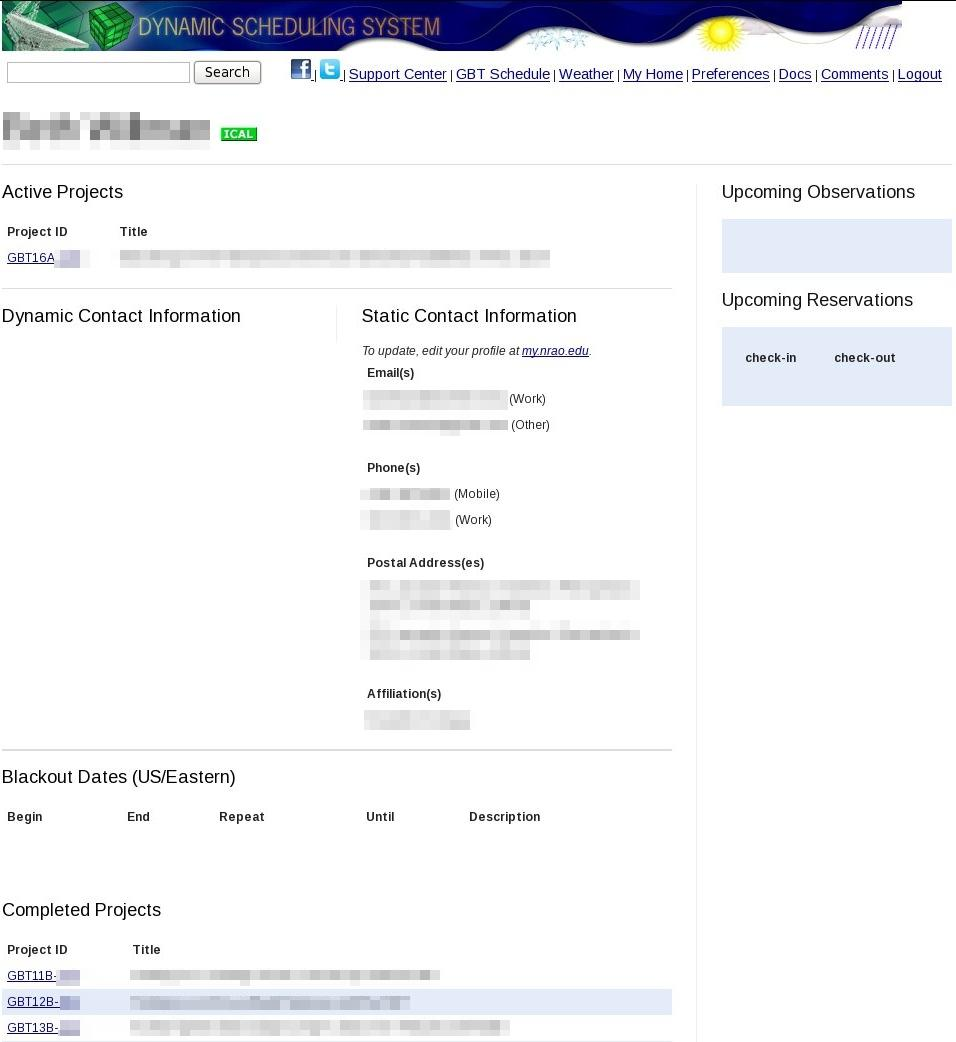
\includegraphics[width=0.6\linewidth]{dss_home_page.jpg}}
\caption[A sample DSS home page]
{A sample \gls{DSS} home page.
\label{fig:dsshome}}
\end{center}
\end{figure}

Upon logging in to the \gls{DSS} system, users arrive at their \gls{DSS} home page
(Figure~\ref{fig:dsshome}) where they see a list of active projects on which they
appear as co-investigator. From the \gls{DSS} home page, users can:
\begin{itemize}[itemsep=1pt]
\item Access the project page for each of their affiliated projects
\item See a list of upcoming observations
\item See a list of upcoming Green Bank room reservations
\item See their {\it static} contact information, as entered in the \gls{NRAO}
      services system \htmladdnormallink{http://my.nrao.edu}{http://my.nrao.edu}.
\item Set {\it dynamic} contact information
\item Set blackout dates
\item Follow a link to the current \gls{GBT} fixed schedule
\item Follow a link to the weather forecasts page
\item follow a link to the \gls{NRAO} support center
\item Set the default time zone via the Preferences link
\item Access \gls{DSS} documentation
\item Establish an iCalendar subscription. Instructions for using iCalendar are available
by hovering the mouse cursor over the iCal icon on the \gls{DSS} Home Page.
\end{itemize}

\newpage

\subsection{The DSS Project Page}

By selecting a project ID, observers are presented with the project page,
where they can:

\noindent\begin{minipage}{0.6\linewidth}
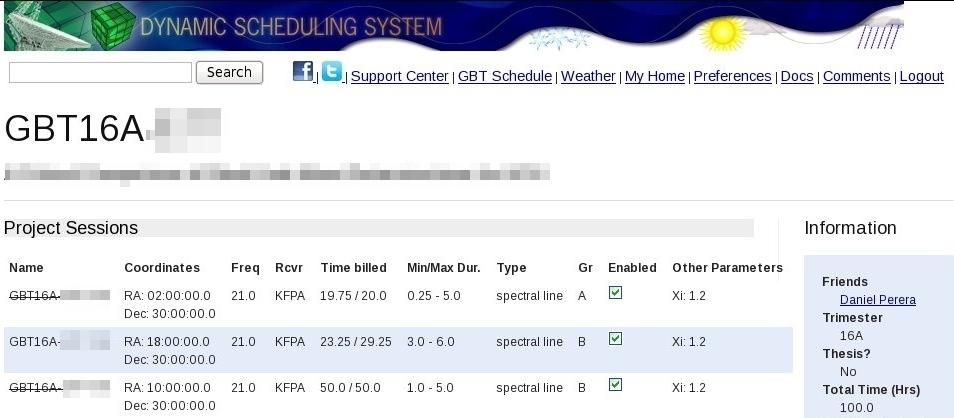
\includegraphics[width=\linewidth]{dss_project_page1.jpg}
\end{minipage}\hfill
\begin{minipage}{0.385\linewidth}
\begin{itemize}[leftmargin=*]
\vspace{2cm}
\item Inspect session parameters
\item Enable or disable individual session
\item View total allocated and billed time
\end{itemize}
\end{minipage}

\noindent\begin{minipage}{0.6\linewidth}
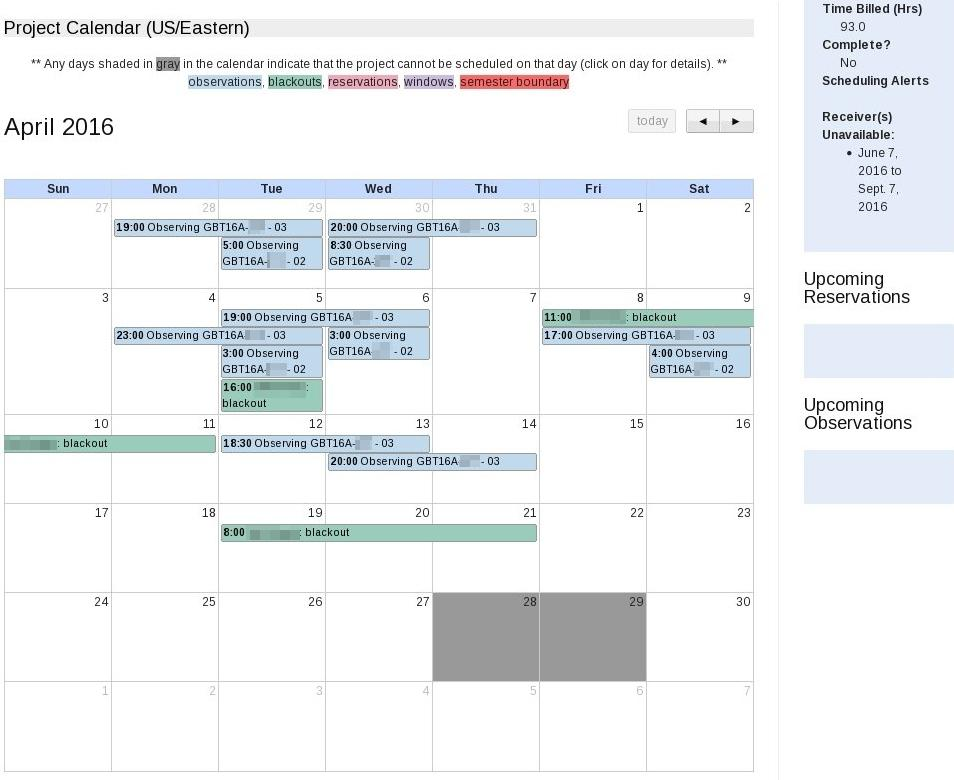
\includegraphics[width=\linewidth]{dss_project_page2.jpg}
\end{minipage}\hfill
\begin{minipage}{0.385\linewidth}
\begin{itemize}[leftmargin=*]
\item See a project calendar
\item View scheduling alerts
\vspace{1.5mm}
\item View receiver availability  %cos minipage is stoopid - or me
\vspace{9mm}
\item View upcoming reservations
\vspace{5mm}
\item View upcoming observations
\vspace{2.8cm}

\end{itemize}
\end{minipage}

\noindent\begin{minipage}{0.6\linewidth}
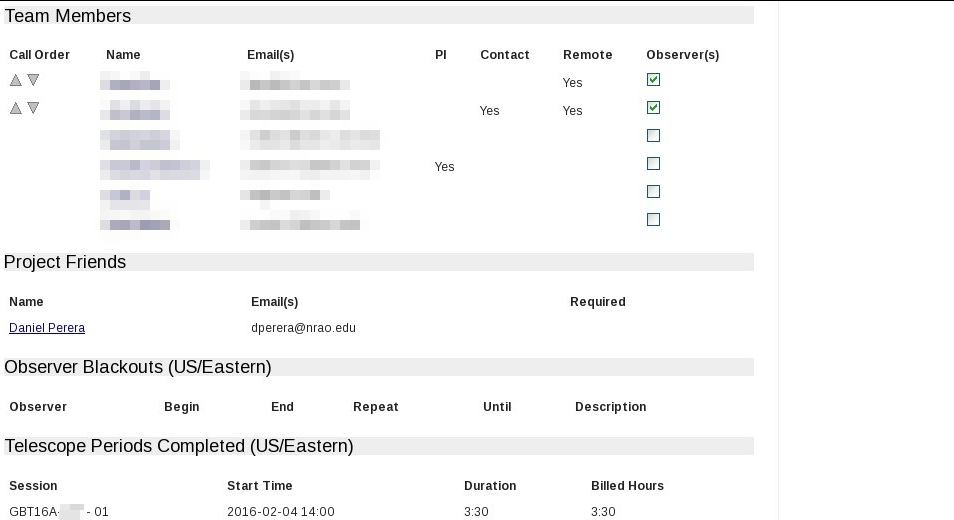
\includegraphics[width=\linewidth]{dss_project_page3.jpg}
\end{minipage}\hfill
\begin{minipage}{0.385\linewidth}
\begin{itemize}[leftmargin=*,itemsep=0pt]
\vspace{5mm}
\item Specify observers from the project team, and set the order they should
      be contacted by \gls{GBT} operations
\vspace{1.3cm}
\item See a list of blackout dates for all\newline observers on the project
\item See a list of completed telescope\newline periods
\end{itemize}
\end{minipage}

\noindent\begin{minipage}{0.6\linewidth}
\setlength{\abovecaptionskip}{-5pt}
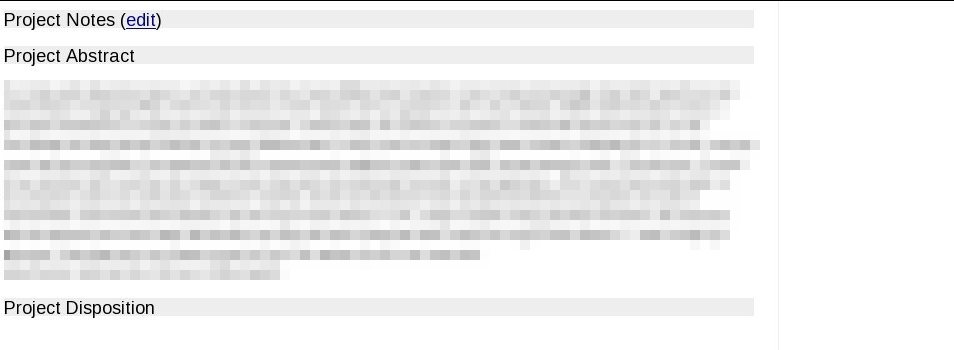
\includegraphics[width=\linewidth]{dss_project_page4.jpg}
\captionof{figure}[A sample DSS project page]{A sample DSS project page.}
\label{fig:dss_project_page}
\end{minipage}\hfill
\begin{minipage}{0.385\linewidth}
\begin{itemize}[leftmargin=*]
\item Store and share project notes
\item View your abstract and disposition
\vspace{2.5cm}
\end{itemize}
\end{minipage}

\newpage


The project calendar gives observers an idea when their project is eligible for scheduling.
Regardless of the weather, there will be times when a project is not eligible for
scheduling, for example because of no receiver availability, observer blackouts, fixed
telescope maintenance periods, and other fixed projects appearing on the \gls{GBT} schedule.
Times not eligible for scheduling will be grayed out on the project calendar.

The project calendar helps with planning in a number of ways. However, it is important
to understand that a session's eligibility is based on ever-changing constraints, and
can change from {\it not eligible} to {\it eligible} at any time. Therefore, if
observers wish to take a break from observing based on the calendar outlook, they
should either disable all sessions until they are ready to resume with the observing,
or enter blackout dates to cover the period they do not wish to observe.

The project page includes a panel with project team members listed. Using a checkbox,
team members can select or deselect those identified as observers. They can also
rearrange the order observers are listed. The top observer in the list is expected to
observe the next scheduled session. If there is a change in schedule, this person will be
called first.

\section{Responsibilities}

Each project has a \glsfirst{PI} and, optionally, a list of additional
investigators. An investigator is eligible to be an observer for a given project if
that person is qualified for remote observing or is on site in Green Bank.

It is essential that one of the observers for a scheduled project contact \gls{GBT}
operations at least 30 minutes prior to the start of the observation. Observers can
contact the \gls{GBT} operator by telephone (304-456-2341), by the \gls{CLEO} chat
program \dq{Talk and Draw}  (for qualified remote observers), or by showing up in
the \gls{GBT} control room. If the \gls{GBT} operator has not been contacted before
the session's start time, the operator will phone observers in the order they are
listed on their project web page.

\begin{itemize}[leftmargin=*]
\item The \gls{PI} is responsible for:\\
\vspace{-5mm}
\begin{itemize}[itemsep=1pt]
\item Managing the project
\item Identifying all associated observers
\item Working with project team members and the \gls{GBT} project Friend to ensure that
\glspl{SB} are properly and promptly prepared.
\item Enabling each session by clicking the \dq{enable} button on the project's web page.
Sessions should be enabled only if they will be ready for observing in the next 24 hours.
\item Ensuring that all associated observers have provided contact information,
including a current telephone number and an email address for each observer.
\item Ensuring that a project's scheduling information is current. This includes
checking the hours remaining on the project and ensuring that the session
parameters are up-to-date and accurate.
\item Ensuring that each scheduled telescope period has an observer who is available at
least 30 minutes before the session is scheduled to begin.
\end{itemize}
\item Observers are responsible for:\\
\vspace{-5mm}
\begin{itemize}[itemsep=1pt]
\item Ensuring that the \gls{DSS} project web page has their current contact information. For
remote observers, this includes entering telephone numbers where they can be
reached at the time of observation.
\item Contacting \gls{GBT} operations 30 minutes prior to the start time of an observation.
\item Attending to observations during a scheduled telescope period.  The \gls{PI} is responsible
for \dq{no-shows} and the ensuing reduction in their alloted time. 
\item Notifying \gls{GBT} operations if they find conditions unsuitable for their session.
\end{itemize}
\end{itemize}

\section{Remote Observing }

% The policies and instructions relating to remote observing remain the same. 
To use the \gls{GBT} remotely, observers must first be trained and certified by Green
Bank staff. In general, astronomers must observe at least once in Green Bank before
being certified for remote observing. {\bf Please note that students should be trained
on site by \gls{GBT} staff, not off site by others}. Experienced observers, when using instruments
or observing modes unfamiliar to them, should plan to visit Green Bank if they require
assistance. 

Contact your project \dq{friend} or the \gls{DSS} helpdesk (helpdesk-dss@gb.nrao.edu) if
you believe the \gls{DSS} does not have you listed properly as a qualified remote observer.

See \htmladdnormallink
{https://science.nrao.edu/facilities/gbt/observing/remote-observing-with-the-gbt}
{https://science.nrao.edu/facilities/gbt/observing/remote-observing-with-the-gbt} and
Chapter~\ref{chap:remote} and for more information on remote observing.


\section{The Daily Schedule}

Each day between about 7:00 and 12:00 PM ET the telescope schedule is fixed for the
24-hour period beginning 8:00 AM ET the next day. For example, by 12:00 PM
Monday, the observing schedule is fixed for the period 8:00 AM Tuesday through 8:00
AM Wednesday. Each morning this daily schedule is published and can be viewed on
the \gls{DSS} web site by anyone. Those with projects on the 24-hour fixed schedule will be
notified by email.

Observers must ensure that their blackout dates and \dq{session enabled} flags are up to date
each day by about 5:00 AM ET. Changes made after this time may not be reflected in the
upcoming day's schedule.

It is possible that weather conditions may change after a schedule is published,
compromising the observing efficiency for some scheduled telescope periods. The
observer or \gls{GBT} staff may then decide to cancel a telescope period and substitute an
alternate \dq{backup} observation in its place. Note that the observer may decide that the
weather conditions are too poor even after beginning the observation. Equipment failure
can also lead to cancellations. If \gls{GBT} staff must change the 24-hour schedule for these
reasons, affected observers will be notified immediately by email or telephone.


\section{Backup Projects}

When a scheduled telescope period is cancelled, a backup project will be scheduled on short notice.
By volunteering as a backup project, observers improve their project's chances of getting
observing time.  Backup projects can come in two categories: observer-run and operator-run.
There are several requirements that must be met before a project can be considered for backup
status. Please refer to Appendix~\ref{appendix:backupprojects} for further details.


\section{Session Types}


There are four types of sessions defined for astronomy projects: open, windowed, elective, and
fixed. Open sessions have no major constraints on when they can be scheduled, beyond
the functional requirements that an observer is available, the source is above the horizon,
and the weather is suitable. Most sessions fall into this category and provide the most
flexibility in the \gls{DSS}. At the other extreme are fixed sessions that have no flexibility
and are prescheduled at a particular date/time; that is, their telescope periods have already
been defined.

The other two types are windowed and elective sessions, which have some constraints but are
not fixed on the schedule. The most common examples are monitoring and \gls{VLBI} sessions,
where the science demands that an object must be observed at defined intervals or times.

Windowed sessions are defined by a cadence that may be either periodic or irregular. For
example, an observer may require observing a target once per month for five months, with
each observation having a tolerance of plus or minus 3 days. In this example, the window
size is 7 days.

Currently, windowed sessions are scheduled in the following way. The cadence information
from the proposal is used to preschedule all windowed sessions whereby all of the
telescope periods are temporarily fixed in what are called default periods. The user is
given the window template (e.g, 8-14 January; 8-14 February; 8-14 March; 8-14 April;
and 8-14 May). Within a windowed period, a windowed session will be considered like
an open session. Near the end of each window range is a default period. If the session
has not been selected by the time the default period arrives, the session will be scheduled
in the default period. The default period may be moved manually to a later time slot
within the window if the human scheduler notices a problem with the original default
period. When the windowed period is scheduled, the observer will be informed 24-48
hours in advance, just like an open session. The only difference is that the observer will
be provided with the window template for planning purposes.

Elective sessions are a restrictive form of windowed sessions.  Here, rather than having a
range of days on which the project session can be scheduled, there is a list of possible days.
As with windows the list of possible days, or {\it opportunities}, has a default period on
which the session will be scheduled if it has not run in advance of that date.

\vspace{-5mm}

\section{Projects that can Tolerate Degraded Weather}

\vspace{-5mm}

The \gls{DSS} is designed to schedule projects in weather that is appropriate for the
frequency being observed. Some projects can tolerate lesser weather conditions than the
\gls{DSS} would assign by default. For example, consider a project at \gls{Kband} that
observes many targets, each for a short duration, say 10 seconds. The observing time for
this project is dominated by overheads in slewing from one position to the next, so
marginal \gls{Kband} weather might be acceptable. The observing team may prefer not to
wait for very good \gls{Kband} weather, which is rare and would delay their scheduling.

To enable more aggressive scheduling, the observer should send an email to the \gls{DSS}
helpdesk requesting that the project be considered for scheduling in lesser weather
conditions. The \gls{DSS} support team can enter a session-specific factor ($\xi$) that
effectively elevates the score for this session in marginal opacity conditions. The $\xi$
parameter is tunable so the observer can request that the project be scheduled very
aggressively, or modestly so. The factor only affects scoring related to atmospheric
opacity, so high frequency projects that are sensitive to high winds will still not get
scheduled when the forecasted winds preclude accurate pointing.

The \gls{DSS} support team will help observers decide if their project can tolerate lesser
weather. Note that this capability will not be used to accelerate scheduling of projects
that truly do benefit from the most appropriate weather.

\section{Other DSS Control Parameters}

A list of the most relevant parameters can be found in
Appendix~\ref{appendix:dsscontrolparameters}. There are a number of additional controls
and parameters that can be used within the DSS system which are fully described in
\gls{DSS} project note 10 (\htmladdnormallink
{https://safe.nrao.edu/wiki/pub/GB/Dynamic/DynamicProjectNotes/dspn10\_6\_final.pdf}
{https://safe.nrao.edu/wiki/pub/GB/Dynamic/DynamicProjectNotes/dspn10\_6\_final.pdf}).
Any changes to these parameters must be requested by contacting the GBT scheduler via
the helpdesk (helpdesk-gb@nrao.edu)

